\documentclass{standalone}
\usepackage{ tikz }
\usepackage{ xparse }
\input{macros/all}

\begin{document}
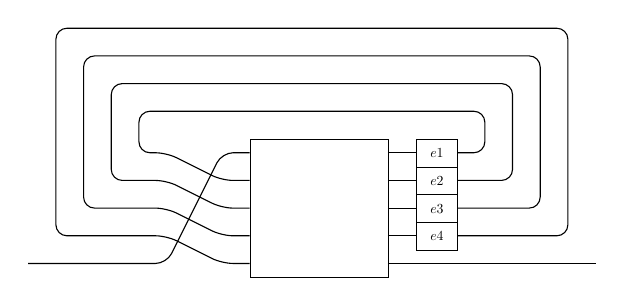
\begin{tikzpicture}[yscale=-1,x=1em,y=1em]

    % wires to shuffle

    \draw [rounded corners] (0,5) -- (5,5) -- (7,1) -- (8,1);
    \draw [rounded corners] (8,5) -- (7,5) -- (5,4) -- (1,4) -- (1,-3.5) -- (19.5, -3.5) -- (19.5, 4) -- (15.5, 4);
    \draw [rounded corners] (8,4) -- (7,4) -- (5,3) -- (2,3) -- (2, -2.5) -- (18.5, -2.5) -- (18.5, 3) -- (15.5,3);
    \draw [rounded corners] (8,3) -- (7,3) -- (5,2) -- (3,2) -- (3,-1.5) -- (17.5, -1.5) -- (17.5, 2) -- (15.5, 2);
    \draw [rounded corners] (8,2) -- (7,2) -- (5,1) -- (4,1) -- (4, -0.5) -- (16.5,-0.5) -- (16.5, 1) -- (15.5, 1);
    
    % shuffle to edges

    \draw [rounded corners] (13,5) -- (20.5,5);
    \draw [rounded corners] (13,4) -- (14,4);
    \draw [rounded corners] (13,3) -- (14,3);
    \draw [rounded corners] (13,2) -- (14,2);
    \draw [rounded corners] (13,1) -- (14,1);

    \node[draw,minimum width=5em,minimum height=5em,anchor=north west] at (8,0.5){$\shufflefun$};
    \node[draw, minimum width = 1.5em, minimum height = 1em, anchor=north west] at (14,0.5){\scalebox{0.5}{$e1$}};
    \node[draw, minimum width = 1.5em, minimum height = 1em, anchor=north west] at (14,1.5){\scalebox{0.5}{$e2$}};
    \node[draw, minimum width = 1.5em, minimum height = 1em, anchor=north west] at (14,2.5){\scalebox{0.5}{$e3$}};
    \node[draw, minimum width = 1.5em, minimum height = 1em, anchor=north west] at (14,3.5){\scalebox{0.5}{$e4$}};
\end{tikzpicture}
\end{document}